% Werke X/1 (1917), native196–200, printed189–193.
\begingroup
\setlength{\headheight}{25pt}
\makeatletter\tagsleft@true\let\veqno\@@leqno\makeatother
\SourceLeaf{196}\ArithmeticHead{189}{R}{\scriptsize EVOLUTIO MEDIORUM ARITHMETICO-GEOMETRICORUM.}
{\small\begin{equation}\tag*{[29]}\left\{\begin{aligned}
&\frac{\partial\log.\left(\frac14s+\frac1{16}s^3+\left[\frac{17}{512}s^5+.\,.\right]\right)}{\partial s}\\
&\quad=\frac{1+\frac34[s^2]+\frac{85}{128}[s^4]+\frac{315}{512}[s^6]\ldots}
{s+\frac14[s^3]+\frac{17}{128}[s^5]+\frac{45}{512}[s^7]\ldots}\\
&\quad=\left[\frac1s\right]\left(1+\frac12[s^2]+\frac{13}{32}[s^4]+\frac{23}{64}[s^6]\ldots\right)
\end{aligned}\right.\end{equation}}
\NumberedItem{6}
\noindent [S. 13]
\[\begin{aligned}
x&=x\\
x'&=(x+\surd(xx-1))^2
\end{aligned}\]
{\small\[\begin{array}{rr|rr|rr}
\varphi&M\sin\varphi&\varphi&M\sin\varphi&\varphi&[M\sin\varphi]\\
0&0&&&&\\
5&0{,}4099431&35&0{,}7719980&65&0{,}9525779\\
10&0{,}5009995&40&0{,}8115373&70&0{,}9696118\\
15&0{,}5674713&45&0{,}8472130.8&75&0{,}9828890\\
20&0{,}6271771&50&0{,}8791266&80&0{,}9923894\\
25&0{,}6803557&55&0{,}9073216&85&0{,}9980965\\
30&0{,}7283955&60&0{,}93180839162&90&1{,}0000000
\end{array}\]}
\ClosingRule
\begin{equation}\tag*{[30]}\left\{\begin{aligned}
Me^x&=1+\frac12x+\frac3{16}xx+\frac5{96}x^3+\frac{11}{1024}x^4+\ldots\\
e^{-\frac12x}Me^x&=1+\frac1{16}xx+\frac1{3072}x^4+\frac{23}{737280}x^6+\ldots\\
&=M\frac12\left(e^{\frac12x}+e^{-\frac12x}\right)
\end{aligned}\right.\end{equation}
\begin{equation}\tag*{[31]}\text{Si statuitur }M\sin\varphi=A-\alpha\cos2\varphi-\beta\cos4\varphi-\text{etc.}\end{equation}
\clearpage
\SourceLeaf{197}\ArithmeticHead{190}{L}{ANALYSIS.\quad NACHLASS.}
\[\begin{array}{r|r}
\text{pro }\varphi=&\text{Erit }A-\gamma\cos2\varphi-\zeta\cos4\varphi\\
0^0&0{,}6212056\\
15&0{,}7566142\\
30&0{,}7832460\\
45&0{,}7991911\\
60&0{,}8103679\\
75&0{,}8168167\\
90&0{,}8189303
\end{array}\]
\[\frac1{M\sin60^0}=1{,}0731820072.\]
\ClosingRule
\NumberedItem{7}
\noindent [S. 13]
\begin{equation}\tag*{[32]}\frac14s+\frac1{16}s^3+\frac{17}{512}s^5+\ldots=z\end{equation}
\begin{equation}\tag*{[33]}\text{1)}\quad Ps=1+4zz+4z^4\quad *\quad+4z^8\end{equation}
\begin{equation}\tag*{[34]}=(2z+2z^9+2z^{25}+\ldots)^2+(1+2z^4+2z^{16}+\ldots)^2\end{equation}
\begin{equation}\tag*{[35]}\text{2)}\quad sPs=2(2z+2z^9+\ldots)\times(1+2z^4+2z^{16}+\ldots)\end{equation}
\begin{equation}\tag*{[36]}Px=1+\frac14xx+\frac{1.9}{4.16}x^4+\text{etc.}\end{equation}
\begin{equation}\tag*{[37]}Mc=\frac1{Ps}\end{equation}
{\small\begin{equation}\tag*{[38]}Ms=\frac{\pi}{-2Ps\times\log.\left(\frac14s+\frac1{16}s^3+\frac{17}{512}s^5+\frac{45}{2048}s^7+\frac{18893}{196608}s^9\right)}\end{equation}}
\begin{equation}\tag*{[39]}\begin{aligned}
\frac{Pc}{Ps}&=-\frac2\pi\log.\left(\frac14s+\frac1{16}s^3+\text{etc.}\right)\\
&=-\frac2\pi\log.\left(\frac14t-\frac1{16}t^3+\frac{17}{512}t^5-\frac{45}{2048}t^7+\text{etc.}\right).
\end{aligned}\end{equation}
\clearpage
\SourceLeaf{198}\ArithmeticHead{191}{R}{\scriptsize EVOLUTIO MEDIORUM ARITHMETICO-GEOMETRICORUM.}
\NumberedItem{8}
\noindent [S. 14]
\begin{equation}\tag*{[40]}\text{Ponendo }P\cos\varphi=N+a\cos2\varphi+b\cos4\varphi+\text{etc.}\end{equation}
\noindent erit
\[\begin{aligned}
N&=1{,}393203\\
a&=0{,}581803\\
b&=0{,}309601\\
c&=0{,}209449\\
d&=0{,}157960\\
e&=0{,}126704
\end{aligned}\]
\[\begin{aligned}
-\frac1\pi\log.(1-\cos2\varphi)&=+0{,}220635\\
&\phantom{=}+0{,}636620\cos2\varphi\\
&\phantom{=}+0{,}318310\cos4\varphi\\
&\phantom{=}+0{,}212207\cos6\varphi\\
&\phantom{=}+0{,}159155\cos8\varphi\\
&\phantom{=}+0{,}127324\cos10\varphi
\end{aligned}\]
\[\begin{aligned}
a&=\frac12\left(\frac{5.5}{4.6}.\frac{9.9}{8.10}.\frac{13.13}{12.14}\text{ etc. in inf.}\right)^2\\
b&=\frac29N\\
N&=\left(\frac{3.3.7.7.11.11.15}{2.4.6.8.10.12.14}\text{ etc. in inf.}\right)^2
=2\frac{\varpi\varpi}{\pi\pi}
\end{aligned}\]
\[2aN=\frac{16}{\pi\pi}\qquad a=\frac4{\varpi\varpi}\]
\[\frac{\varpi}{\surd8}=\frac{4.6.8.10.12.14}{5.5.9.9.13.13}\text{ etc.}\]
\[\frac{\varpi}2=\frac32.\frac45.\frac76.\frac89.\frac{11}{10}.\frac{12}{13}\ldots\]
\NumberedItem{9}
{\small\begin{equation}\tag*{[41]}\begin{aligned}
&1+\left(\frac12\right)^3x^2+\left(\frac12.\frac34\right)^3x^4
+\left(\frac12.\frac34.\frac56\right)^3x^6+\text{etc.}\\
&=\left(1+\left(\frac14\right)^2x^2+\left(\frac14.\frac58\right)^2x^4
+\left(\frac14.\frac58.\frac9{12}\right)^2x^6+\text{etc.}\right)^2.
\end{aligned}\end{equation}}
\clearpage
\SourceLeaf{199}\ArithmeticHead{192}{L}{ANALYSIS.\quad NACHLASS.}
\begin{center}\textit{Demonstratio.}\end{center}
\par\indent Ponatur
\[1+\left(\frac14\right)^2x^4+\left(\frac14.\frac58\right)^2x^8+\text{etc.}=t\]
\noindent eritque, posito
\[x(x^4-1)\frac{d^2t}{dx^2}+(3x^4-1)\frac{dt}{dx}+x^3t=R,\]
\[R=0.\]
\noindent Hinc etiam
\[0=x\frac{dR}{dx}+R;\]
\noindent nec non
\[0=2xt\frac{dR}{dx}+2\left(t+3x\frac{dt}{dx}\right)R,\]
\noindent unde fit (evolutione facta)
{\small\[\begin{aligned}
0={}&xx(x^4-1)\left(2t\frac{d^3t}{dx^3}+6\frac{dt}{dx}.\frac{d^2t}{dx^2}\right)\\
&+3x(3x^4-1)\left(2t\frac{d^2t}{dx^2}+2\frac{dt}{dx}.\frac{dt}{dx}\right)\\
&+(19x^4-1)2t\frac{dt}{dx}+8x^3tt
\end{aligned}\]}
\noindent sive ponendo \(tt=u\)
{\small\[0=xx(x^4-1)\frac{d^3u}{dx^3}+3x(3x^4-1)\frac{d^2u}{dx^2}
+(19x^4-1)\frac{du}{dx}+8x^3u,\]}
\noindent cui aequationi invenitur respondere
\[u=1+\left(\frac12\right)^3x^4+\left(\frac{1.3}{2.4}\right)^3x^8+\text{etc.}\]
\noindent [S. 15]
\par\indent Iam quum
\[t=\frac{\surd8}{\pi}\int\frac{dz}{{}^{4}\!\surd(1-z^4)(1-x^4z^4)}\]
\noindent a \(z=0\) usque ad \(z=1\), fit, pro \(x=1\),
\[t=\frac{\surd8}{\pi}.\frac{\varpi}2=\frac{\varpi}{\pi}\surd2\]
\noindent adeoque
\[1+\left(\frac12\right)^2+\left(\frac{1.3}{2.4}\right)^3+\left(\frac{1.3.5}{2.4.6}\right)^3+\ldots
=2\frac{\varpi\varpi}{\pi\pi}.\]
\clearpage
\SourceLeaf{200}\ArithmeticHead{193}{R}{\scriptsize EVOLUTIO MEDIORUM ARITHMETICO-GEOMETRICORUM.}
\begin{center}\textit{Idem alio modo.}\end{center}
\par\indent Valor seriei
\[1+\left(\frac12\right)^3+\left(\frac{1.3}{2.4}\right)^3+\left(\frac{1.3.5}{2.4.6}\right)^3+\text{etc.}\]
\noindent fit
\[=\frac4{\pi\pi}\int\int\frac{d\varphi\,d\psi}{\surd(1-\cos\varphi^2\cos\psi^2)}\]
\noindent a \(\varphi=0\) usque ad \(\varphi=90^0\) et a \(\psi=0\) usque ad \(\psi=90^0\).
\par\indent Faciendo itaque
\[\cos\varphi\cos\psi=\cos v,\]
\noindent idem valor fit
\[=\frac4{\pi\pi}\int\int\frac{d\varphi\,dv}{\surd(\cos\varphi^2-\cos v^2)}\]
\noindent et quidem ab \(v=0\) usque ad \(v=90^0\) et a \(\varphi=0\) usque ad \(\varphi=v\). Denique statuendo
\[\varphi+v=f,\ v-\varphi=g\]
\noindent erit expressio nostra
\[=\frac2{\pi\pi}\int\int\frac{df\,dg}{\surd\sin f.\sin g}\]
\noindent a \(g=0\) usque ad \(g=90^0\) et ab \(f=g\) usque ad \(f=180^0-g\).
Sed haud difficulter probatur integrale eundem valorem nancisci, si sumatur ab \(f=0\) usque ad \(f=90^0\) et a \(g=0\) usque ad \(g=90^0\), unde ipsius valor deducitur
\[=2\frac{\varpi\varpi}{\pi\pi},\]
\noindent uti supra.
\begin{flushright}
\begin{tikzpicture}[x=.012cm,y=-.012cm,line width=.65pt]
\draw (38,41)--(167,160)--(167,283)--(38,283)--cycle;
\draw (38,283)--(167,160);
\draw (38,51)--(49,51);
\draw (38,62)--(61,62);
\draw (38,71)--(71,71);
\draw (38,79)--(79,79);
\draw (38,89)--(90,89);
\draw (38,99)--(101,99);
\draw (38,106)--(109,106);
\draw (38,115)--(118,115);
\draw (38,124)--(128,124);
\draw (38,132)--(137,132);
\draw (38,142)--(148,142);
\draw (38,150)--(157,150);
\draw (38,159)--(166,159);
\draw (38,167)--(160,167);
\draw (38,177)--(149,177);
\draw (38,185)--(141,185);
\draw (38,195)--(130,195);
\draw (38,203)--(122,203);
\draw (38,214)--(110,214);
\draw (38,222)--(102,222);
\draw (38,232)--(91,232);
\draw (38,242)--(81,242);
\draw (38,251)--(72,251);
\draw (38,259)--(63,259);
\draw (38,268)--(54,268);
\draw (38,276)--(45,276);
\node[anchor=east,font=\small] at (37,40) {180};
\node[anchor=east,font=\small] at (36,167) {90};
\node[anchor=east,font=\small] at (36,219) {\(f\)};
\node[anchor=north,font=\small] at (103,284) {\(g\)};
\node[anchor=north west,font=\small] at (165,284) {90};
\end{tikzpicture}
\end{flushright}
\ClosingRule
\clearpage
\endgroup

